\documentclass[a4paper 12pt]{article}

\usepackage[utf8]{inputenc}
\usepackage[T1]{fontenc}
\usepackage{mathptmx}
\usepackage{textcomp}
\usepackage[UKenglish]{babel}
\usepackage{amsmath, amssymb}
\usepackage{float}
\usepackage{xcolor}
\definecolor{codegreen}{rgb}{0,0.6,0}
\definecolor{codepurple}{rgb}{0.58,0,0.82}
\usepackage{listings}
\lstdefinestyle{code}{
	commentstyle=\color{codegreen},
	keywordstyle=\color{magenta},
	stringstyle=\color{codepurple},
	showspaces=false,
	showstringspaces=false,
	breaklines=true
}
\lstset{style=code}
\usepackage[hidelinks]{hyperref}
\hypersetup{
	colorlinks=false
}
\usepackage[style=ieee]{biblatex}
\bibliography{sources/biblio}
\renewcommand{\baselinestretch}{1.5}

\setlength{\parindent}{0pt}
\setlength{\parskip}{1em}

% figure support
\usepackage{import}
\usepackage{xifthen}
\pdfminorversion=7
\usepackage{pdfpages}
\usepackage{transparent}
\newcommand{\incfig}[1]{%
	\def\svgwidth{\columnwidth}
	\import{./figures/}{#1.pdf_tex}
}

\pdfsuppresswarningpagegroup=1

\begin{document}
\hypersetup{pageanchor=false}
\begin{titlepage}
  \begin{center}

    \textsc{\LARGE Dublin City University}\\[1cm]
    \textsc{\Large Electronic and Computer Engineering}\\[0.5cm]

    {\LARGE \bfseries EE513 Connected Embedded Systems\\[0.4cm]}
    {\Large \bfseries Assignment 1\\[0.4cm]}

    \begin{figure}[H]
	
\includegraphics{images/Dcu-logo.png}
	\centering
    \end{figure}

    \vskip 2cm
    \emph{Author}\\[0.1cm]
    \noindent\makebox[\textwidth]{%
      \begin{tabular}{ll}%
        Michael Lenehan & michael.lenehan4@mail.dcu.ie \\
	Student Number: & 15410402 \\
    \end{tabular}}\\[0.1cm]

    \vfill

    % Bottom of the page
    % Probably replaced with date of deadline
    {\large{09/03/2020}}

  \end{center}
\end{titlepage}

\hypersetup{pageanchor=true}
\pagenumbering{alph}
\thispagestyle{plain}
\begingroup
\renewcommand{\cleardoublepage}{}
\renewcommand{\clearpage}{}

\LARGE{Declaration}

\endgroup

\vskip 1cm

I declare that this material, which I now submit for assessment, is entirely my
own work and has not been taken from the work of others, save and to the extent
that such work has been cited and acknowledged within the text of my work. I
understand that plagiarism, collusion, and copying are grave and serious
offences in the university and accept the penalties that would be imposed should
I engage in plagiarism, collusion or copying. I have read and understood the
Assignment Regulations set out in the module documentation. I have identified
and included the source of all facts, ideas, opinions, and viewpoints of others
in the assignment references. Direct quotations from books, journal articles,
internet sources, module text, or any other source whatsoever are acknowledged
and the source cited are identified in the assignment references. This
assignment, or any part of it, has not been previously submitted by me or any
other person for assessment on this or any other course of study.

I have read and understood the DCU Academic Integrity and Plagiarism at
\url{https://www4.dcu.ie/sites/default/files/policy/1%20-%20integrity_and_plagiarism\_ovpaa_v3.pdf}
and IEEE referencing guidelines found at
\url{https://loop.dcu.ie/mod/url/view.php?id=448779}.

\vskip 1cm
Signed: \underline{\ \ \ \ \ \ \ \ \ \ \ \ \ \ \ \ \ \ \ \ \ \ \ \ \ \ \ \ \ \ \
\ \ \ \ \ \ } \hspace{20mm}Date: \underline{09/03/2020}

\hspace*{0mm}\phantom{Signed:}Michael Lenehan

\pagebreak

\pagenumbering{arabic}
\thispagestyle{plain}
\begin{center}
    \Large
    \textbf{Title}

    \vspace{0.4cm}
    \large
    Subtitle

    \vspace{0.4cm}
    \textbf{Michael Lenehan}

    \vspace{0.9cm}
    \textbf{Abstract}

\end{center}

\par

\pagebreak

\tableofcontents
\clearpage
\section{Introduction}
This assignment aims to introduce students to integrating physical sensors or
devices with an embedded Linux platform. In this case the physical device being
used is the DS3231 Real Time Clock module, and the embedded Linux platform is a
Raspberry Pi 3 Model B+. The devices can communicate via the I2C protocol.

The requirements of the assignment state that a C++ class must be implemented
for this integration. This class must contain all methods required for the reading
and writing of the RTC time, date, alarm, control, and temperature registers.
The student must also implement a ``novel function'' of their choosing.

In completing this assignment, the student should have a greater understanding
of the object oriented code required for I2C communications, and the code
required to read or write data to/from a physical devices registers.

\section{Assignment Setup}
\subsection{RTC Circuit}
The following components are used for this assignment:

\begin{enumerate}
	\item Raspberry Pi 3 Model B+
	\item Samsung SD Card
	\item Maxim Integrated DS3231 Real Time Clock Breakout Board.
\end{enumerate}

The I2C protocol is used for communications between the RTC and the Raspberry
Pi. As such, the RTC must be connected to the Raspberry Pi via the I2C data and
clock connections, on pins 3 and 5 (GPIO 2 and 3) respectively. The RTC breakout
board operates on a 3.3V supply voltage, and as such the 3.3V (pin 1), and
ground (pin 6) pins must also be connected.

Connecting these pins results in the following layout:

\begin{figure}[H]
	\centering
	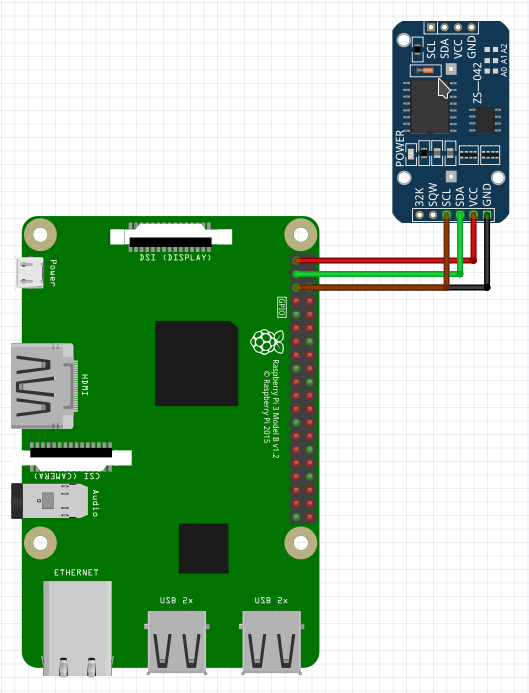
\includegraphics[width=0.45\textwidth, angle=90]{images/circuit}
	\caption{I2C connection from RTC to Raspberry Pi}
	\label{fig:i2c}
\end{figure}

The physical circuit appears as follows:

\subsection{I2C Discovery and Testing}
In order to setup I2C on the Raspberry Pi 3 Model B+, the I2C bus must first be
enabled. This is achieved by executing the command ``raspi-config''. Navigating
to the ``Interfacing Options'' tab, and selecting ``I2C'' to enable the bus.

Once the circuit is connected, the i2ctools package must be installed in order
to verify the connection. The package can be installed by executing the
following command:

\begin{lstlisting}[language=bash]
	sudo apt install i2c-tools
\end{lstlisting}

Once installed the I2C bus can be scanned using the ``i2cdetect command''. The
``-l'' option lists the installed busses.

\begin{lstlisting}[language=bash]
	i2cdetect -l
\end{lstlisting}

The output of this command corresponds to the I2C bus that the device is
connected to. Using the ``-r'' option, bus 1 can be scanned using
the SMBus ``receive byte'' method. The ``-y'' option in this case disables user
input for confirmation.

\begin{lstlisting}[language=bash]
	i2cdetect -y -r 1
\end{lstlisting}

Finally the ``i2cdump'' command can be used to dump the contents of the
specified address, in this case ``0x68'' on bus 1:

\begin{lstlisting}[language=bash]
	i2cdump -y 1 0x68
\end{lstlisting}

\section{C++ Code}
\subsection{Reading Time and Date}
To read the time and date, the I2C bus connection must be opened, the device
address must be connected to, the read address must be specified, and the values
must be read into a buffer.
This functionality was implemented within the ``I2CDevice'' class. The
``setupProc'' method calls the ``openBus'', ``connectDevice'', ``resetReadAddr''
and ``readBuffer'' methods each time an object of the I2CDevice class is
created, opening the connection to the device.

\lstinputlisting[language=C++, caption={setupProc Function}]{snippets/setupProc.cpp}

From the read buffer, the desired values can be displayed. This functionality is
implemented using the ``DS3231'' class ``readTimeAndDate'' method:

\lstinputlisting[language=C++, caption={readTimeAndDate Function}]{snippets/readTandD.cpp}

This method reads from the registers indexed by values `2', `1', and `0', which
are the hours, minutes, and seconds registers respectively, printing their
values in decimal form. As the values read from these registers are in binary
coded decimal format, the provided ``bcdToDec'' function is used to convert
them. The date values are read from registers `4', `5', and `6', which are the
day, month and year registers respectively. These values are also stored in BCD
format, and so the ``bcdToDec'' function must be used for the purpose of
printing.

\subsection{Reading Temperature}
The temperature value can be read from the RTC in much the same way as the time,
however, the values within the temperature registers are stored in two's
compliment representation, with the upper two bits of the least significant bits
register representing a ratio of the degree value. With a precision of $\pm$
0.25 degrees, the LSB bits can represent a 0.00 degrees (bits 00), 0.25 degrees
(bits 01), 0.50 degrees (bits 10), and 0.75 degrees (bits 11).

\lstinputlisting[languag=C++, caption={readTemp Function}]{snippets/temp.cpp}

In order to extract the upper two bits of a byte, a bitwise right shift by 6
places is used. Multiplying 100 by the new value and dividing by 4 gives the
degrees ratio value. This can then be printed to the screen. The temperature MSB
value is stored in the register indexed `17' with the LSB in the register
indexed `18'.

\subsection{Setting Time and Date}
In order to write values to the RTC, a write function must be implemented. As
the write procedure is generic to I2C devices, this function was added to the
``I2CDevice'' class.

\lstinputlisting[language=C++, caption={writeToReg Function}]{snippets/write.cpp}

This function takes a register number and an input value. The register value is
then used as the address at which to begin writing the new value.

For the DS3231, the time and date must be written in Binary Coded Decimal. As
such a ``decToBCD'' function was implemented. This function takes an input
character representing a decimal value, and outputs a BCD encoded value.

\lstinputlisting[language=C++, caption={decToBCD Function}]{snippets/decToBCD.cpp}

The time values can then be written to the corresponding registers. The time and
date registers are as described above. The table in Figure
\ref{fig:images-timeDateRegisters} shows the bits for each of the registers, and
the functions of each bit.

\begin{figure}[H]
	\centering
	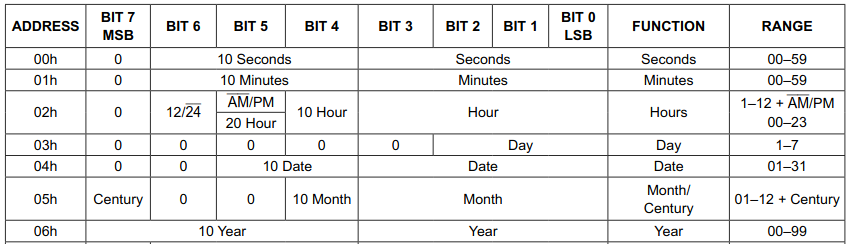
\includegraphics[width=0.8\textwidth]{images/timeDateRegisters}
	\caption{Time and Date Register Layout}
	\label{fig:images-timeDateRegisters}
\end{figure}

The code in Listing \ref{lst:writeTimeDate} shows the ``writeTime'' and
``writeDate'' functions, which pass the input character array values to the
``writeToReg'' function in order to be written to the RTC. As the upper nibble
of the ``Hours'' register contain control bits, these bits must not be modified
during a write operation. The ``hrRegChangeUpperBits'' function modifies only
the LSB of the upper nibble. The ``Dates'' register contains a ``10 Date''
value, to which a value is assigned using the ``dateChangeUpperBits'' function.
A check is used within the ``writeDate'' function to test if the date value is
within the appropriate range.

\lstinputlisting[language=C++, caption={writeTime and writeDate Functions}, label={lst:writeTimeDate}]
{snippets/writeTimeDate.cpp}

\subsection{Setting Alarms and Interrupts}
Reading and setting the alarms works in much the same way as reading and writing
the time, and the alarm values are also stored in BCD encoded format. In
order to read the value of the alarms, the values in registers 7, 8, 9 and 10
can be printed. For alarm 2 the values in registers 11, 12 and 13 can be
printed. As these are stored in BCD format, the bcdToDec function
needs to be called.

Writing the alarms works in a similar manner to writing the time and date,
however as the upper bits of each register contains control bits, care must be
taken not to unintentionally overwrite the values within these positions. Again,
the decToBCD function is required to be used to convert the values to binary
coded decimal. Should this function not be called, the alarm values will not
match the time values, and the interrupt cannot be triggered. A bitwise
``clear'' operation is used in order to clear the ``Alarm Mask'' bits. This
allows the interrupt condition to be due to a match in date, seconds, minutes,
and hours.

\begin{figure}[H]
	\centering
	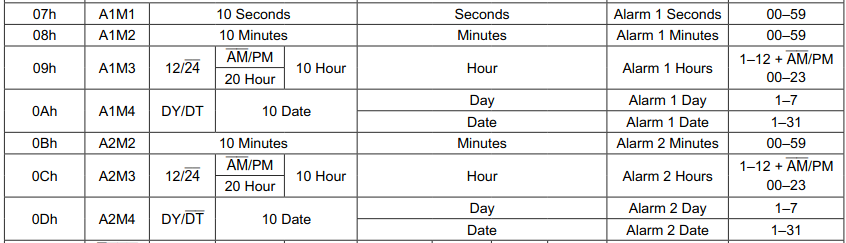
\includegraphics[width=0.8\textwidth]{images/alarmRegisters}
	\caption{Alarm 1 and Alarm 2 Registers}
	\label{fig:images-alarmRegister}
\end{figure}

\lstinputlisting[language=C++, caption={writeAlarm Function}]{snippets/writeAlarm.cpp}

The interrupt can be set by setting the $3^{rd}$ bit of the control register high.
This bit controls the square wave generator output, and, as such, setting the
bit high will disable the output when the interrupt alarm condition is met. The
``setInterrupt'' function takes two boolean inputs, which are used to confirm
setting the ``A1E'' and ``A2E'' alarm enable bits. If either boolean is true,
the interrupt bit is set high, along with the bit of the corresponding alarm. If
neither boolean is true, the interrupt bit is set low. Once all of the required
bits are set/cleared using the ``changeBits'' function, the value within the
buffer can be written to the register.

\begin{figure}[H]
	\centering
	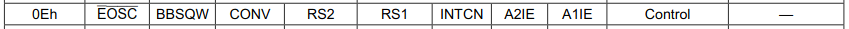
\includegraphics[width=0.8\textwidth]{images/controlRegister}
	\caption{Control Register}
	\label{fig:images-controlRegister}
\end{figure}

\lstinputlisting[language=C++, caption={set Interrupt Function}]{snippets/setInterrupt.cpp}

\subsection{Novel Functionality}
For the novel functionality, it was decided that it would be a useful feature to
be able to initialize the RTC time based on the current system time. This was
done using a combination of file I/O operations, and a system call to the Linux
``date'' utility. This utility allows for the formatting of the output based on
a number of input arguments. In this case the arguments ``+\%S \%M \%H \%u \%d \%m
\%Y'' specify to output the seconds, minutes, hours, weekday number, date, month,
and year, delimited by spaces.

The output of the ``date'' command is passed into a temporary file, ``tmp'' from
which it can be read, with the symbols delimited by the whitespace. The values
are placed in a string vector via the ``push\_back'' method. The temporary file
is then closed and deleted. The vector values are converted to integers using
the ``stoi'' function, and placed in separate time and date character arrays,
from which they can be passed into the ``writeTime'' and ``writeDate''
functions.

\lstinputlisting[language=C++, caption={Novel Function - Initialize RTC time
from System Time}, label={lst:novel}]{snippets/novel.cpp}

\section{Linux Kernel Module}
This section of the assignment implements a Linux Kernel Module in order to read
and write the RTC time. The ``rtc-ds1307.ko'' LKM is compatible with the DS3231,
and will be used for this section. The Linux ``modprobe'' program is used to add
the LKM to the kernel. The ds1307 device is then instantiated by writing its
address to the i2c-1 directories ``new\_device'' file. This process can be seen
in Figure \ref{fig:images-lkm1}.

\begin{figure}[H]
	\centering
	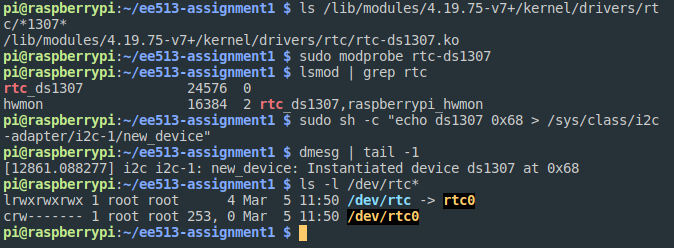
\includegraphics[width=0.8\textwidth]{images/lkm1}
	\caption{Adding the DS1307 LKM to the Kernel}
	\label{fig:images-lkm1}
\end{figure}

Executing the ``i2cdetect'' command shows a value of ``UU'' at the RTC's
address, showing the device is in use by an LKM.

\begin{figure}[H]
	\centering
	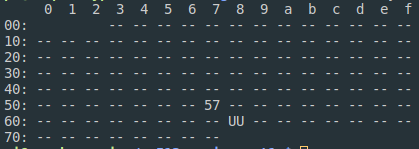
\includegraphics[width=0.8\textwidth]{images/lkm2}
	\caption{i2cdetect Output}
	\label{fig:images-lkm2}
\end{figure}

By navigating to the devices ``sysfs'' entry, the ``cat'' command can be used to
output the current RTC time to the user.

\begin{figure}[H]
	\centering
	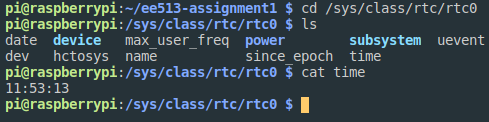
\includegraphics[width=0.8\textwidth]{images/lkm3}
	\caption{RTC output via the ``cat'' command}
	\label{fig:images-lkm3}
\end{figure}

The ``hwclock'' utility can also be used to read or write to the RTC, with the
``set'' option allowing for the system time to be set from the RTC.

\begin{figure}[H]
	\centering
	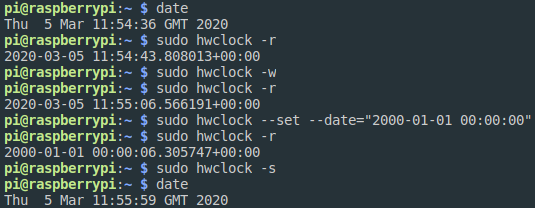
\includegraphics[width=0.8\textwidth]{images/lkm4}
	\caption{``hwclock'' utility usage}
	\label{fig:images-lkm4}
\end{figure}

To automatically set the time via the RTC at boot time, a systemd service can be
added to the ``system'' directory. The contents of this service file can be seen
in Figure \ref{fig:images-lkm5}.

\begin{figure}[H]
	\centering
	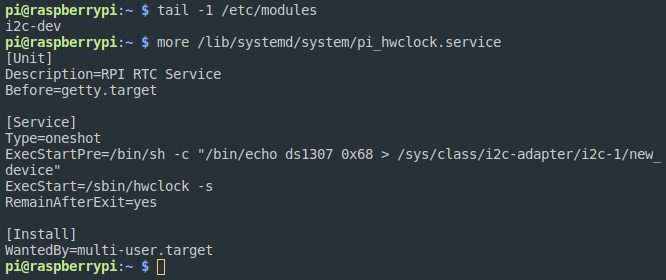
\includegraphics[width=0.8\textwidth]{images/lkm5}
	\caption{System service integration}
	\label{fig:images-lkm5}
\end{figure}

In order to start this service, the ``systemctl'' command can be run. The NTP
service must also be disabled, however, as shown in Figure \ref{fig:images-lkm6}, the
``ntp'' service is not available. This is because it is no longer included in
the Raspbian Stretch images.

\begin{figure}[H]
	\centering
	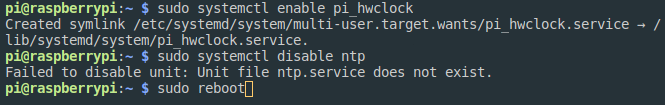
\includegraphics[width=0.8\textwidth]{images/lkm6}
	\caption{Enabling the system service}
	\label{fig:images-lkm6}
\end{figure}

Once the system has been rebooted, the status of this system service can be
checked. Figure \ref{fig:images-lkm7} shows that the service is active after a
reboot.

\begin{figure}[H]
	\centering
	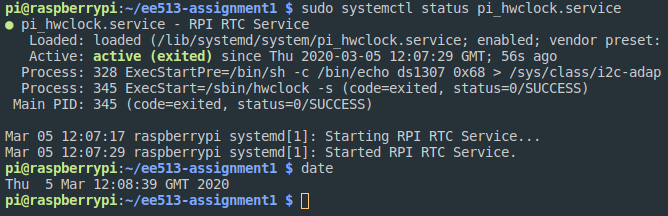
\includegraphics[width=0.8\textwidth]{images/lkm7}
	\caption{System service status}
	\label{fig:images-lkm7}
\end{figure}

Finally, in order to remove the LKM and undo the creation of the system service,
the service must be disabled, with the ntp service re-enabled. As mentioned,
this service no longer exists within the Raspbian Stretch images. The LKM can
then be removed by passing the RTC address (0x68) to the ``delete\_device'' file
of the ``i2c-1'' directory. This can be verified using the ``i2cdetect''
command, which shows the address 0x68 for the RTC, indicating it is no longer in
use by the LKM.

\begin{figure}[H]
	\centering
	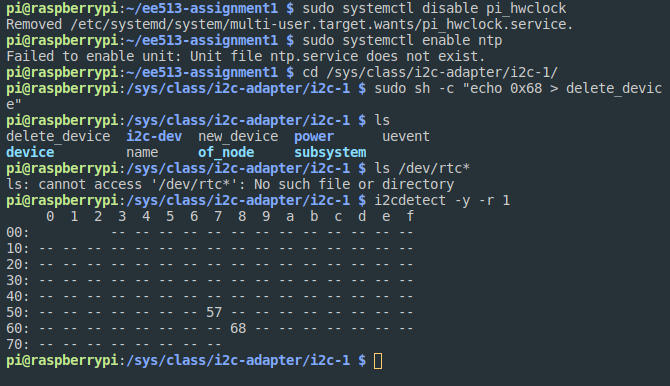
\includegraphics[width=0.8\textwidth]{images/lkm8}
	\caption{Removing the LKM and freeing the RTC}
	\label{fig:images-lkm8}
\end{figure}

\section{Conclusion}
Each of the required read and write functions of the assignment were implemented.
The novel functionality was also implemented. Documentation was created
using ``Doxygen'' and can be found in the submit git repository.

Figures \ref{fig:images-git1} and \ref{fig:images-git2} show the GitLab commit
history for the assignment. This does not demonstrate the full history of the
project, as a number of merged branches were later deleted, however all major
changes are reflected in the screenshots.

\begin{figure}[H]
	\centering
	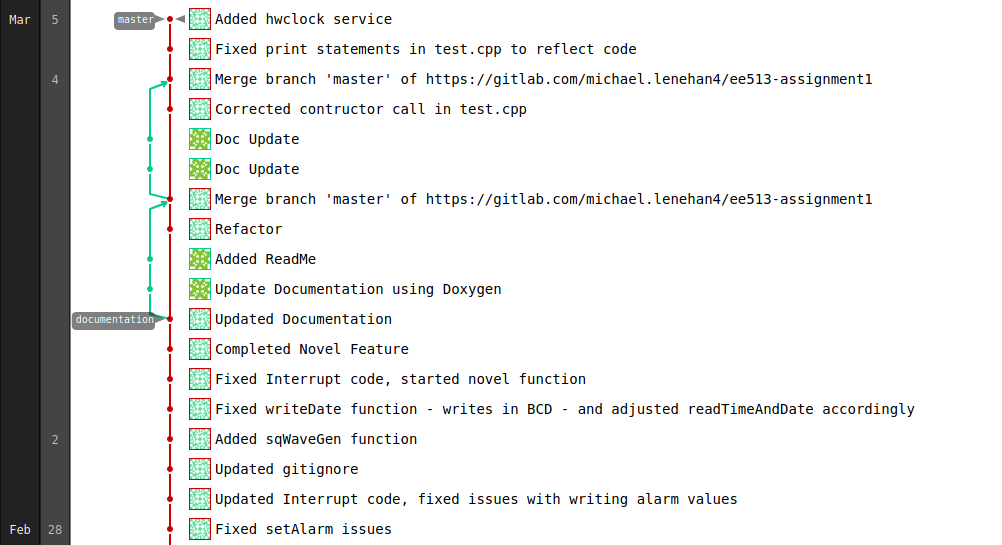
\includegraphics[width=0.8\textwidth]{images/git1}
	\caption{GitLab Commit History}
	\label{fig:images-git1}
\end{figure}

\begin{figure}[H]
	\centering
	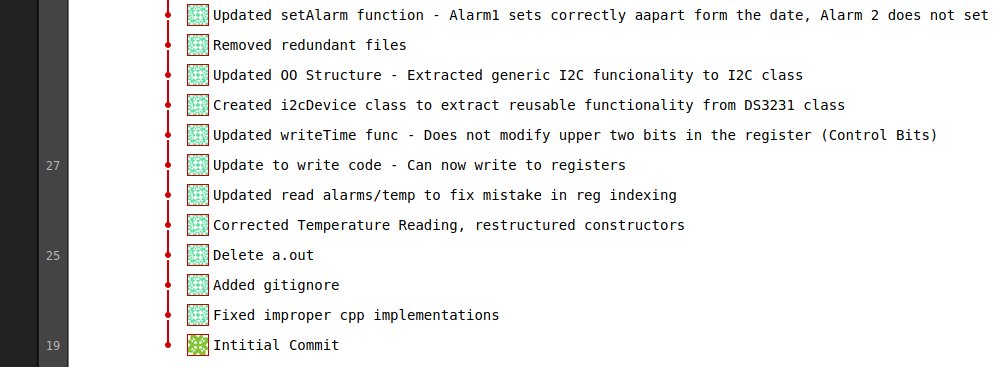
\includegraphics[width=0.8\textwidth]{images/git2}
	\caption{GitLab Commit History}
	\label{fig:images-git2}
\end{figure}

The interrupt
did not operate as expected. Reading the datasheet indicates that the interrupt
bit being set high while the alarm flag is low would result in no output on the
square wave output, however the exact opposite is true, with no output on the
pin only if the alarm flag is high.

Overall a lot was learned with regards to integrating hardware with an embedded
Linux system, including how to communicate via I2C, and how to perform
integration testing.

\clearpage
\printbibliography
\end{document}
